\section{Resultados e comparações}
\begin{table}[H]
\centering\small
\setlength{\tabcolsep}{3.7pt}
\caption{Média das cinco partições externas, com pesos iguais. DP é o desvio-padrão entre
partições, não um intervalo de confiança. Menores erros e maiores precisões
são melhores. As duas ordenações do KNN compartilham as previsões de nota.}
\label{tab:resultados}
\begin{tabular}{@{}lrrrr@{}}
\toprule
Modelo & RMSE $\pm$ DP & MAE & $P$@10 $\pm$ DP & nDCG@10\\
\midrule
\tblAtivResultados
\bottomrule
\end{tabular}
\end{table}

O \textbf{SVD é o melhor estimador de notas}: reduz o RMSE em \ganhoRmse\% em
relação ao KNN e o supera nas cinco partições. Também produz listas melhores
que o KNN ordenado por nota prevista. A variante por soma inverte o resultado
do ranking: alcança \somaP\ de precisão, equivalente a \acertosSoma\ acertos por lista,
contra \acertosSvd\ do SVD e \acertosPop\ da popularidade.

\begin{figure}[H]
\centering
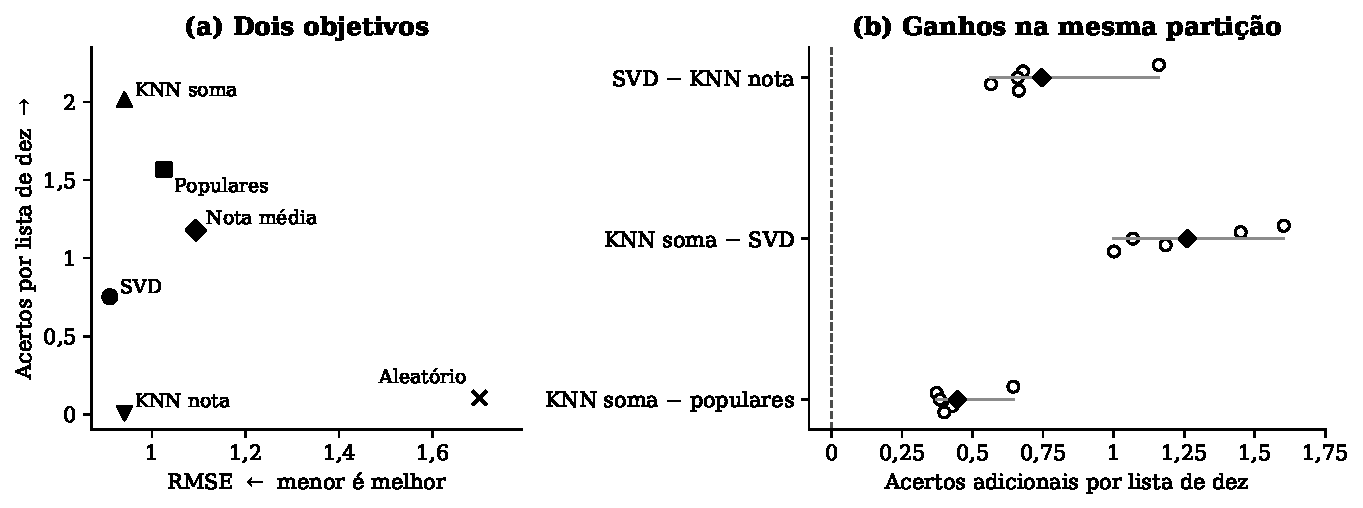
\includegraphics[width=\textwidth]{figuras/ativ_comparacoes.pdf}
\caption{(a) Posição dos modelos nos dois objetivos: o canto superior esquerdo
combina menor erro com mais acertos. (b) Ganhos de acertos por lista, sempre
comparando métodos na mesma partição. Cada círculo representa uma das cinco
partições; o losango é a média e o segmento mostra a amplitude, sem inferência
estatística. Valores positivos favorecem o primeiro método.}
\label{fig:comparacoes}
\end{figure}

\textbf{A vantagem sobre um modelo simples é menor que a vantagem sobre o SVD.}
O KNN por soma acrescenta \difSomaSvd\ acerto por lista em relação ao SVD, mas \difSomaPop\ em
relação à popularidade, um ganho relativo de \ganhoPop\%. Essa segunda
comparação dimensiona o benefício além de simplesmente recomendar filmes
muito avaliados. Os ganhos são positivos nas cinco partições.

O resultado aleatório fica próximo da expectativa exata \acasoP, calculada
pela fração de filmes relevantes entre candidatos, nos mesmos usuários
da comparação.

Com os mesmos vizinhos, a regra de ordenação muda radicalmente a precisão.
O diagnóstico seguinte examina essa diferença sem alterar as configurações.
